% !TeX program = xelatex
\documentclass[10pt, a4paper]{article}

\newif\ifpeerreview
\peerreviewfalse % Set \peerreviewtrue for anonymous Pintia peer-review submission

\usepackage{amsmath, amssymb, amsthm, mathtools}
\usepackage{geometry}
\usepackage{fancyhdr}
\usepackage{enumitem}
\usepackage{titlesec}
\usepackage{tocloft}
\usepackage[x11names]{xcolor}
\usepackage{graphicx}
\usepackage{float}
\usepackage{booktabs}
\usepackage{array}
\usepackage{multirow}
\usepackage{caption}
\usepackage{subcaption}
\usepackage{tikz}
\usepackage{microtype}
\usepackage{listings}
\usepackage[most]{tcolorbox}
\tcbuselibrary{skins, breakable}
\usepackage[backend=biber, citestyle=numeric-comp, bibstyle=numeric]{biblatex}
\usepackage{hyperref}
\usepackage{xurl}
\usepackage[capitalise, noabbrev]{cleveref}

\usetikzlibrary{arrows.meta, calc, positioning}

% --- Palette: Navy + Amber Gold + Sage ---
\definecolor{primary}{RGB}{28, 55, 90}
\definecolor{accent}{RGB}{176, 128, 52}
\definecolor{accentlight}{RGB}{232, 214, 178}
\definecolor{problembg}{RGB}{250, 248, 243}
\definecolor{problemframe}{RGB}{210, 220, 232}
\definecolor{textmuted}{RGB}{95, 105, 118}
\definecolor{coverbg}{RGB}{252, 249, 238}
\definecolor{progcolor}{RGB}{52, 105, 88}
\definecolor{bonuscolor}{RGB}{129, 86, 165}

% --- Page Geometry & Header/Footer ---
\geometry{left=2.4cm, right=2.4cm, top=2.6cm, bottom=2.6cm}
\setlength{\headheight}{18pt}
\setlength{\parindent}{1.5em}
\setlength{\parskip}{0.38em}
\linespread{1.15}
\emergencystretch=2em
\setlist{nosep, leftmargin=1.8em}

\pagestyle{fancy}
\fancyhf{}
\fancyhead[L]{\small\color{primary}\textsf{ADS Project 4: Improving Dynamic Programming for Knapsack}}
\fancyhead[R]{\small\color{textmuted}\textsf{Fall--Winter 2026}}
\fancyfoot[C]{\small\color{textmuted}\thepage}
\renewcommand{\headrulewidth}{0.5pt}
\renewcommand{\headrule}{%
  {\color{accent!55}\hrule width\headwidth height 0.5pt}%
}

% --- Section & Subsection Headings ---
\titleformat{\section}
  {\color{primary}\centering\Large\bfseries}
  {\color{accent}Chapter~\thesection.}{0.6em}{}
  [\vspace{0.3em}{\color{accent!70}\titlerule[1.5pt]}]

\titleformat{name=\section,numberless}
  {\color{primary}\centering\Large\bfseries}
  {}{0pt}{}
  [\vspace{0.3em}{\color{accent!70}\titlerule[1.5pt]}]

\titleformat{\subsection}
  {\color{primary!88!black}\large\bfseries}
  {\color{accent}\thesubsection}{0.6em}{}
  [\vspace{0.15em}{\color{accent!45}\titlerule[0.8pt]}]

\titleformat{\subsubsection}
  {\color{primary!85!black}\normalsize\bfseries}
  {\color{accent}\thesubsubsection}{0.5em}{}

\titlespacing*{\section}{0pt}{0.6em}{1.0em}
\titlespacing*{\subsection}{0pt}{1.0em}{0.6em}
\titlespacing*{\subsubsection}{0pt}{0.8em}{0.4em}

% --- TOC Styling ---
\renewcommand{\cftsecfont}{\bfseries\color{primary}}
\renewcommand{\cftsecpagefont}{\bfseries\color{primary}}
\renewcommand{\cftsubsecfont}{\color{black!85}}
\renewcommand{\cftsubsubsecfont}{\small\color{textmuted}}
\setlength{\cftbeforesecskip}{0.55em}

% --- Styled Boxes ---
\newtcolorbox{theorembx}[1]{
    enhanced,
    breakable,
    colback=problembg,
    colframe=primary!30,
    boxrule=0.7pt,
    arc=3.5pt,
    borderline west={3.2pt}{0pt}{primary},
    left=12pt,
    right=12pt,
    top=7pt,
    bottom=8pt,
    before skip=7pt plus 2pt,
    after skip=8pt plus 2pt,
    title={\sffamily #1},
    fonttitle=\bfseries,
    coltitle=white,
    colbacktitle=primary,
    attach boxed title to top left={yshift=-2mm, xshift=8mm},
    boxed title style={
        arc=2.2pt,
        boxrule=0pt,
        top=1.8pt,
        bottom=1.8pt,
        left=6pt,
        right=6pt,
    },
}

\newtcolorbox{lemmabx}[1]{
    enhanced,
    breakable,
    colback=accentlight!22,
    colframe=accent!45,
    boxrule=0.65pt,
    arc=3.5pt,
    borderline west={3.0pt}{0pt}{accent!80},
    left=12pt,
    right=12pt,
    top=7pt,
    bottom=8pt,
    before skip=7pt plus 2pt,
    after skip=8pt plus 2pt,
    title={\sffamily #1},
    fonttitle=\bfseries,
    coltitle=primary,
    colbacktitle=accentlight!85,
    attach boxed title to top left={yshift=-2mm, xshift=8mm},
    boxed title style={
        arc=2.2pt,
        boxrule=0.5pt,
        colframe=accent!55,
        top=1.8pt,
        bottom=1.8pt,
        left=6pt,
        right=6pt,
    },
}

\newtcolorbox{insightbox}[1]{
    enhanced,
    breakable,
    colback=progcolor!5.5,
    colframe=progcolor!28,
    boxrule=0.7pt,
    arc=4pt,
    borderline west={3.5pt}{0pt}{progcolor},
    left=13pt,
    right=13pt,
    top=8pt,
    bottom=9pt,
    before skip=8pt plus 2pt,
    after skip=9pt plus 2pt,
    title={\sffamily #1},
    fonttitle=\bfseries,
    coltitle=white,
    colbacktitle=progcolor,
    attach boxed title to top left={yshift=-2mm, xshift=8mm},
    boxed title style={
        arc=2.5pt,
        boxrule=0pt,
        top=2pt,
        bottom=2pt,
        left=7pt,
        right=7pt,
    },
}

% --- Code Listings & Captions ---
\newcommand{\code}[1]{\texttt{\color{primary!90!black}#1}}
\newcommand{\kw}[1]{\textbf{\color{primary}#1}}
\newcommand{\id}[1]{\ensuremath{\mathrm{#1}}}
\captionsetup{labelfont={bf,color=primary}, skip=4pt}
\BeforeBeginEnvironment{tabular}{\small}

\lstset{
    language=C,
    basicstyle=\ttfamily\scriptsize,
    keywordstyle=\color{primary}\bfseries,
    commentstyle=\color{progcolor}\itshape,
    stringstyle=\color{accent},
    breaklines=true,
    numbers=left,
    numberstyle=\tiny\color{textmuted},
    frame=single,
    rulecolor=\color{problemframe},
    backgroundcolor=\color{problembg},
    captionpos=b,
    tabsize=4,
    columns=fullflexible,
    showstringspaces=false
}

\hypersetup{
    colorlinks=true,
    linkcolor=primary,
    citecolor=progcolor,
    urlcolor=accent,
    linktoc=all,
    pdfauthor={},
    pdftitle={Improving Dynamic Programming for the 0/1 Knapsack Problem}
}

\graphicspath{{../src/visualizations/}{../plots/}{image/}{figure/}}
\addbibresource[location=local]{reference.bib}

\begin{document}

% ============================================================
%  PAGE 1: DEDICATED COVER + ABSTRACT PAGE
% ============================================================
\begin{titlepage}
\begin{tikzpicture}[remember picture, overlay]
    \fill[coverbg] (current page.south west) rectangle (current page.north east);
    \draw[accent!40, line width=0.7pt]
        ([xshift=1.5cm, yshift=-1.5cm]current page.north west) --
        ([xshift=1.5cm, yshift=1.5cm]current page.south west);
    \draw[accent!40, line width=0.7pt]
        ([xshift=-1.5cm, yshift=-1.5cm]current page.north east) --
        ([xshift=-1.5cm, yshift=1.5cm]current page.south east);
    \foreach \r in {2.0, 2.45, 2.9} {
        \draw[primary!14, line width=0.5pt]
            ([xshift=-1.35cm, yshift=1.35cm]current page.south east) circle (\r cm);
        \draw[primary!14, line width=0.5pt]
            ([xshift=1.35cm, yshift=-1.35cm]current page.north west) circle (\r cm);
    }
\end{tikzpicture}

\vspace*{0.7cm}
\begin{center}
    {\large\color{accent}\textsf{\textbf{Advanced Data Structures and Algorithm Analysis}}}\\[0.25cm]
    {\normalsize\color{textmuted}\textsf{Laboratory Project Report $\cdot$ Project 4}}\\[0.55cm]

    {\color{primary}\rule{0.58\textwidth}{1.4pt}}\\[0.5cm]
    {\fontsize{22}{29}\selectfont\bfseries\color{primary} Improving Dynamic Programming}\\[0.2cm]
    {\fontsize{22}{29}\selectfont\bfseries\color{primary} for the 0/1 Knapsack Problem}\\[0.45cm]
    {\color{accent}\rule{0.24\textwidth}{1.0pt}}\\[0.5cm]
    \ifpeerreview
        {\Large\bfseries\color{accent}\textsf{Group X}}\\[0.65cm]
        {\Large\bfseries\color{primary} Student A \hspace{2.8em} Student B}\\[0.35cm]
    \else
        {\Large\bfseries\color{accent}\textsf{Group 15}}\\[0.65cm]
        {\Large\bfseries\color{primary} Yixiang Chen \hspace{2.8em} Runhui Lin}\\[0.35cm]
    \fi
    {\normalsize\color{textmuted}
        Zhejiang University \\[0.15cm]
        Date: 2026-11-21
    }
\end{center}

\vspace{0.55cm}
\begin{center}
    {\large\bfseries\color{primary} Abstract}
\end{center}
\vspace{-0.25em}
\begin{quote}
\small\noindent
The \textbf{0/1 Knapsack Problem} seeks an item subset of maximum profit within capacity $c$. Standard dynamic programming \textbf{DP-1} takes $\Theta(nc)$ time and space regardless of instance structure. Based on Sections~3.4--3.5 of \emph{The Knapsack Problems} and the $O(n + W^3)$ small-weight algorithm, we implement and compare four exact C11 solvers: dense-table \code{origin}, dominance-pruned state-list \code{list}, fractional-bound-pruned \code{bound}, and bonus \code{w3} for maximum item weight $W = \max_j w_j$, using a BFPRT density prefix, $2W$-proximity window, and SMAWK concave convolution. Under an isolated Windows Job Object harness with a $1\,\text{GiB}$ RAM limit, we run $5{,}257$ trials across KPLIB and controlled synthetic suites with $100\%$ optimal-value agreement. On large-capacity KPLIB instances, \code{list} and \code{bound} achieve $\mathbf{14.2\times\text{--}56.1\times}$ speedups over \code{origin} for $n \le 200$ and solve $n \in \{500, 1000\}$ where \code{origin} exceeds $1\,\text{GiB}$, while per-state $O(n)$ bounding causes \code{list} to outperform \code{bound} by $\mathbf{3.17\times\text{--}6.32\times}$ at $n \ge 500$. At small weight $W = 16$ and $n = 3{,}200$, \code{w3} finishes in $\mathbf{0.72\,\text{ms}}$---$\mathbf{89.6\times}$, $\mathbf{236.3\times}$, and $\mathbf{3{,}750.1\times}$ faster than \code{origin}, \code{list}, and \code{bound}---while degrading rapidly once $W$ becomes large.

\vspace{0.5em}\noindent
{\color{primary}\textbf{Keywords:}} 0/1 knapsack problem; dynamic programming; dominance pruning; fractional knapsack bound; proximity; SMAWK concave convolution.
\end{quote}

\vfill
\begin{center}
    {\color{accent!80}\rule{0.14\textwidth}{0.8pt}}\\[0.25cm]
    {\normalsize\bfseries\color{primary} Fall--Winter 2026}
\end{center}
\end{titlepage}

% ============================================================
%  PAGE 2: DEDICATED TABLE OF CONTENTS PAGE
% ============================================================
\pagenumbering{roman}
\thispagestyle{plain}
\vspace*{0.3cm}
\tableofcontents
\clearpage

% ============================================================
%  CHAPTER 1: INTRODUCTION
% ============================================================
\pagenumbering{arabic}
\section{Introduction}

\subsection{Problem Description}
Given $n$ items with positive integer weights $w_1, \ldots, w_n$, non-negative integer profits $p_1, \ldots, p_n$, and capacity $c$, the \textbf{0/1 Knapsack Problem} computes the maximum achievable profit
\begin{equation}
  z^* \;=\; \max \left\{ \sum_{j=1}^{n} p_j x_j \;\middle|\; \sum_{j=1}^{n} w_j x_j \le c,\;\; x_j \in \{0, 1\} \text{ for } j = 1, \ldots, n \right\}.
  \label{eq:kp}
\end{equation}
In the ADS lectures~\cite{ads_slides2026}, \textbf{DP-1} defines $P[j][d]$---written $z_j(d)$ in Kellerer et al.~\cite{kellerer2004knapsack}---as the maximum profit from the first $j$ items within capacity $d \in \{0, \ldots, c\}$, with $P[0][d] = 0$ and $P[j][d] = -\infty$ for $d < 0$:
\begin{equation}
  P[j][d] \;=\; \max\bigl\{\, P[j-1][d],\;\; P[j-1][d - w_j] + p_j \,\bigr\}, \qquad 1 \le j \le n,\;\; 0 \le d \le c.
  \label{eq:dp1}
\end{equation}
Evaluating (\ref{eq:dp1}) always requires $\Theta(nc)$ time and $\Theta(nc)$ table memory, even when most capacities are unreachable or suboptimal. To overcome these bottlenecks while preserving exactness, we study four solvers:
\begin{itemize}
  \item \textbf{\color{primary}Baseline Table DP, \code{origin}:} Fills the dense $(n+1) \times (c+1)$ matrix via (\ref{eq:dp1}) in $\Theta(nc)$ time and space~\cite{ads_slides2026}.
  \item \textbf{\color{primary}DP-with-Lists, \code{list}:} Maintains ordered stage lists $L_j$ of $(w, p)$ pairs and prunes dominated states with $w \le w'$ and $p \ge p'$, achieving $\Theta(n)$ best-case and $O(nB)$ parameterized time~\cite{kellerer2004knapsack}.
  \item \textbf{\color{primary}DP-with-Upper-Bounds, \code{bound}:} Orders items by $p_1/w_1 \ge \cdots \ge p_n/w_n$ and prunes any state whose fractional-knapsack upper bound does not beat the incumbent profit $P^*$~\cite{kellerer2004knapsack}.
  \item \textbf{\color{primary}Bonus Proximity + SMAWK DP, \code{w3}:} Uses a BFPRT density prefix, $2W$-proximity window, and SMAWK concave convolution to run in $O(n + W^3)$ time for $W = \max_j w_j$, independent of $c$~\cite{polak2021knapsack}.
\end{itemize}

\subsection{Purpose of This Report}
This report implements all four exact solvers in C11 and characterizes their empirical regimes across $n$, $c$, and $W$:
\begin{enumerate}[label=\textbf{\color{primary}\arabic*.}]
  \item \textbf{Realize Four Exact Solvers:} Implement \code{knapsack\_list\_with\_bound}, \code{knapsack\_origin}, \code{knapsack\_list}, and bonus \code{knapsack\_w3} under a unified C11 interface, verified by unit and regression tests.
  \item \textbf{Benchmark Complementary Regimes:} Use our Job-Object-isolated harness \code{testbench.c} to evaluate large-capacity KPLIB suites, fixed-capacity synthetic suites, and controlled small-weight and weight-sweep suites.
  \item \textbf{Analyze Complexity and Applicable Regimes:} Analyze the time and space bounds of all four algorithms, explaining the $1\,\text{GiB}$ memory wall of \textbf{DP-1}, the bounding crossover of \code{bound}, and the small-weight regime of \code{w3}.
\end{enumerate}

\clearpage

% ============================================================
%  CHAPTER 2: DATA STRUCTURE AND ALGORITHM SPECIFICATION
% ============================================================
\section{Data Structure and Algorithm Specification}

\subsection{Overview of Solver and Benchmark Data Structures}
\Cref{tab:structures} summarizes the C11 structures across our solver headers and batch benchmark harness \code{testbench.c}. Whereas \code{knapsack\_origin} stores stage $i$ as a dense row \code{best\_solution[i][0..c]}, the list solvers retain only undominated states, and \code{knapsack\_w3} operates on $O(W^2)$ correction arrays and implicit residue matrices.

\begin{table}[H]
\centering
\caption{Core solver and benchmark data structures in \code{src/}.}
\label{tab:structures}
\begin{tabular}{@{}l>{\raggedright\arraybackslash}p{0.33\linewidth}>{\raggedright\arraybackslash}p{0.43\linewidth}@{}}
\toprule
\textbf{\color{primary}Structure} & \textbf{\color{primary}C Fields / Layout} & \textbf{\color{primary}Structural Invariant \& Role} \\
\midrule
\code{State} & \code{int weight}, \code{int profit} & Feasible subproblem pair $(w, p)$ with $w \in [0, c]$; sentinel \code{(INT\_MAX, 0)} marks list end during merging. \\
\code{StateList} & \code{State* data}, \code{int size}, \code{int allocated} & Contiguous array of undominated states satisfying $w_1 < \cdots < w_m$ and $p_1 < \cdots < p_m$. \\
\code{ItemRatio} & \code{int index}, \code{double ratio} & Pairs 0-based item subscript $i$ with density $p_i / w_i$ for non-increasing efficiency sorting. \\
\code{KW3Item} & \code{int p}, \code{int w}, \code{int id} & Usable item record ordered by 64-bit cross product $p_a w_b$ vs.\ $p_b w_a$ with \code{id} tie-breaking. \\
\code{KW3Matrix} & \code{const int64\_t *old}, \code{*gain}; \code{size\_t h}, \code{residue}, \code{count} & Implicit inverse-Monge matrix for weight-$h$ residue $r$, evaluated in $O(1)$ via \code{(distance, base)} pairs. \\
\code{Instance} & \code{int n}, \code{capacity}, \code{max\_weight}, \code{int* profits}, \code{int* weights} & Validated in-memory \code{.kp} instance tracking $W = \code{max\_weight}$ with 32-bit overflow guards. \\
\code{Result} & \code{const char* status}, \code{int profit}, \code{double seconds}, \code{DWORD exit\_code} & Stores isolated worker status, returned optimal profit, and pure QPC solver time. \\
\bottomrule
\end{tabular}
\end{table}

\subsection{Baseline Table-Based Dynamic Programming: \texttt{origin}}
In \code{Knapsack\_origin.h}, \code{knapsack\_origin} allocates an array of $n + 1$ row pointers \code{best\_solution[0..n]}, each pointing to a heap buffer of $c + 1$ \code{int} entries. After initializing the base row $\code{best\_solution}[0][0..c] \gets 0$, two nested loops iterate over $i = 1, \ldots, n$ and $j = 0, \ldots, c$: each cell copies the exclusion value $\code{best\_solution}[i-1][j]$ and, whenever $j \ge w_i$, compares it against the inclusion candidate $\code{best\_solution}[i-1][j - w_i] + p_i$. Once cell $(n, c)$ is computed, all $n + 1$ row buffers and the pointer directory are freed before returning \code{best\_solution[n][c]}. Because standard table-based DP is covered in the ADS lectures~\cite{ads_slides2026}, we omit a separate pseudo-code listing and use \textbf{DP-1} as our empirical baseline.

\subsection{Dynamic Programming with Lists and Dominance Pruning: \texttt{list}}
Following Section~3.4 of Kellerer et al.~\cite{kellerer2004knapsack}, \code{knapsack\_list} replaces dense capacity indexing with an explicit stage list $L_j = \langle (w_{1j}, p_{1j}), \ldots, (w_{m_j,j}, p_{m_j,j}) \rangle$, initialized at $L_0 = \langle (0, 0) \rangle$. Given two feasible states $(w, p)$ and $(w', p')$ in stage $j$, state $(w, p)$ \textbf{dominates} $(w', p')$ if and only if
\begin{equation}
  (w < w' \;\text{and}\; p \ge p') \qquad\text{or}\qquad (w \le w' \;\text{and}\; p > p').
  \label{eq:dominance}
\end{equation}
By optimal substructure, extending a dominated state $(w', p')$ by any subset of remaining items $\{j+1, \ldots, n\}$ uses at least as much weight and yields no greater profit than extending $(w, p)$ by the same subset; duplicate states $(w, p) = (w', p')$ are likewise redundant. Removing all dominated and duplicate pairs leaves a strictly totally ordered list of \textbf{undominated states}:
\[
  0 \;=\; w_{1j} < w_{2j} < \cdots < w_{m_j,j} \;\le\; c
  \qquad\text{and}\qquad
  0 \;=\; p_{1j} < p_{2j} < \cdots < p_{m_j,j}.
\]
Consequently, the maximum profit after $n$ items is always stored at the last element of $L_n$, namely $\code{lists[n].data[lists[n].size - 1].profit}$.

At stage $j$, \code{knapsack\_list} first constructs the shifted candidate list $L'_j = L_{j-1} \oplus (w_j, p_j)$ by adding $(w_j, p_j)$ to each state in $L_{j-1}$; because $L_{j-1}$ is sorted by increasing weight, the scan terminates via \kw{break} at the first state with $w + w_j > c$. Next, \code{Mergelist} appends the sentinel \code{(INT\_MAX, 0)} via \code{add\_sentinel} to both $L_{j-1}$ and $L'_j$, seeds $\code{Merged.data}[0] \gets \code{(INT\_MAX, 0)}$, and repeatedly pops the smaller-weight head state $(w, p)$ until both cursors reach \code{INT\_MAX}. Let $(w_{\text{last}}, p_{\text{last}})$ denote the current tail of \code{Merged}:
\begin{itemize}
  \item \textbf{\color{primary}Dominated / Duplicate Skip:} For any non-zero state with $p \le p_{\text{last}}$, we have $w \ge w_{\text{last}}$, so $(w, p)$ is dominated by $(w_{\text{last}}, p_{\text{last}})$ and discarded in $O(1)$ time.
  \item \textbf{\color{primary}Equal-Weight Tail Replacement:} If $p > p_{\text{last}}$ and $w \le w_{\text{last}}$, $(w, p)$ overwrites the tail slot $\code{Merged.data}[\code{flag\_merged}]$.
  \item \textbf{\color{primary}Undominated State Append:} If $p > p_{\text{last}}$ and $w > w_{\text{last}}$, $(w, p)$ is appended at \code{++flag\_merged} and \code{Merged.size} is incremented.
\end{itemize}

\begin{table}[H]
\centering
\begin{tabular}{@{}p{2.05cm}p{0.78\textwidth}@{}}
\toprule
\multicolumn{2}{@{}l}{\textbf{\color{primary}Algorithm 1:} List-Based DP $\id{knapsack\_list}(n, c, p, w)$ and $\id{Mergelist}(L, L')$ in \code{Knapsack\_List.h}} \\
\midrule
\textbf{DP-Lists:} &
1. Initialize $L_0 \gets \langle (0, 0) \rangle$ with $\code{size} = 1$. \\
& 2. \kw{for} $j = 1$ \kw{to} $n$ \kw{do} \\
& 3. \quad Set $L'_j \gets \langle\,\rangle$. \kw{for} $k = 0$ \kw{to} $|L_{j-1}| - 1$ \kw{do}: let $(w, p) \gets L_{j-1}[k]$; \kw{if} $w + w_j > c$ \kw{then break}; append $(w + w_j, p + p_j)$ to $L'_j$. \\
& 4. \quad $L_j \gets \id{Mergelist}(L_{j-1}, L'_j)$; free temporary buffer $L'_j$. \\
& 5. Save $z^* \gets L_n[|L_n|-1].\id{profit}$, free $L_0, \ldots, L_n$, and \kw{return} $z^*$. \\[0.3em]
\textbf{Mergelist:} &
1. Append sentinel $(\infty, 0)$ to $L$ and $L'$; set $M[0] \gets (\infty, 0)$, $\code{size} \gets 1$, and cursors $i_1 \gets 0, i_2 \gets 0, t \gets 0$. \\
& 2. \kw{repeat} \\
& 3. \quad Pop $(w, p) \gets (L[i_1].w < L'[i_2].w) \mathbin{?} L[i_1\text{++}] : L'[i_2\text{++}]$. \\
& 4. \quad \kw{if} $p > M[t].p$ \kw{or} $(w = 0 \text{ and } p = 0)$ \kw{then} \\
& 5. \quad\quad \kw{if} $w \le M[t].w$ \kw{then} $M[t] \gets (w, p)$ \kw{else} $M[\text{++}t] \gets (w, p)$ and increment $M.\code{size}$. \\
& 6. \kw{until} $L[i_1].w = \infty$ \kw{and} $L'[i_2].w = \infty$; \kw{return} $M$. \\
\bottomrule
\end{tabular}
\end{table}

\subsection{Hybrid List DP with Fractional Knapsack Upper Bounds: \texttt{bound}}
Dominance pruning only compares combinations of the first $j$ items, retaining states that have no chance of reaching the global optimum via the remaining items $\{j+1, \ldots, n\}$. Following Section~3.5 of \emph{The Knapsack Problems}~\cite{kellerer2004knapsack}, \code{knapsack\_list\_with\_bound} combines list-based DP with branch-and-bound upper-bound pruning.

First, \code{selection\_sort} in \code{Fraction\_Knapsack.h} sorts all $n$ items in non-increasing order of unit profit:
\begin{equation}
  \frac{p_1}{w_1} \;\ge\; \frac{p_2}{w_2} \;\ge\; \cdots \;\ge\; \frac{p_n}{w_n}.
  \label{eq:ratio_order}
\end{equation}
For each candidate state $(w, p)$ at stage $j$, \code{fraction\_knapsack} solves the fractional knapsack problem on the remaining items $\{j+1, \ldots, n\}$ with residual capacity $c - w$: whole items are added greedily until the first item $s$ that exceeds the remaining space, giving the integer upper bound
\begin{equation}
  U_j(w, p) \;=\; p + \sum_{\ell=j+1}^{s-1} p_\ell + \left\lfloor \frac{p_s \cdot \bigl(c - w - \sum_{\ell=j+1}^{s-1} w_\ell\bigr)}{w_s} \right\rfloor,
  \label{eq:ub}
\end{equation}
or $p + \sum_{\ell=j+1}^{n} p_\ell$ when all remaining items fit.

Let $P^*$ denote the best feasible profit found so far, initialized to $0$. In \code{Mergelist\_with\_bound}, every popped state $(w, p)$ is checked against $U_j(w, p)$: if $U_j(w, p) \le P^*$, the state is pruned immediately; otherwise, $P^*$ is updated to $\max(P^*, p)$ and $(w, p)$ enters the dominance check. At $j = n$, \code{fraction\_knapsack} returns $0$ so $U_n(w, p) = p \le P^*$, and the solver returns $P^*$. Algorithm~2 and \Cref{fig:pruning_trace} summarize this procedure.

\begin{figure}[H]
\centering
\begin{tikzpicture}[
  x=1.0cm, y=0.86cm,
  font=\scriptsize,
  keepst/.style={draw=progcolor, thick, rounded corners=2pt, fill=progcolor!9, text=primary, inner sep=2.2pt, minimum width=12.5mm, align=center, font=\scriptsize\bfseries},
  domst/.style={draw=textmuted, dashed, rounded corners=2pt, fill=problembg, text=textmuted, inner sep=2.2pt, minimum width=12.5mm, align=center},
  fathst/.style={draw=Red3!80, thick, rounded corners=2pt, fill=Red3!8, text=Red3!90!black, inner sep=2.2pt, minimum width=12.5mm, align=center},
  hdr/.style={font=\scriptsize\bfseries\color{primary}, align=center}
]
  % Column headers
  \node[hdr] at (0.0, 3.35) {$j=0$\\init};
  \node[hdr] at (2.15, 3.35) {$j=1$\\$(2,6)$};
  \node[hdr] at (4.45, 3.35) {$j=2$\\$(2,3)$};
  \node[hdr] at (6.85, 3.35) {$j=3$\\$(6,5)$};
  \node[hdr] at (9.55, 3.35) {$j=4$: $(5,4)$, $P^*\!=18$};
  \node[hdr] at (12.35, 3.35) {$j=5$\\$(4,2)$};

  % j=0
  \node[keepst] (s0) at (0.0, 2.3) {$(0,0)$};

  % j=1
  \node[keepst] (s10) at (2.15, 2.3) {$(0,0)$};
  \node[keepst] (s11) at (2.15, 1.45) {$(2,6)$};

  % j=2
  \node[keepst] (s20) at (4.45, 2.3) {$(0,0)$};
  \node[keepst] (s21) at (4.45, 1.45) {$(2,6)$};
  \node[domst]  (s2d) at (4.45, 0.60) {$(2,3)$};
  \node[keepst] (s22) at (4.45, -0.25) {$(4,9)$};

  % j=3
  \node[fathst] (s3f) at (6.85, 2.3) {$(0,0)$\\[-1pt]{\tiny $U_3\!=\!6$}};
  \node[keepst] (s31) at (6.85, 1.30) {$(2,6)$};
  \node[keepst] (s32) at (6.85, 0.45) {$(4,9)$};
  \node[domst]  (s3d) at (6.85, -0.40) {$(6,5)$};
  \node[keepst] (s33) at (6.85, -1.25) {$(8,11)$};
  \node[keepst] (s34) at (6.85, -2.10) {$(10,14)$};

  % j=4 (two subcolumns: pruned vs kept)
  \node[fathst] (s4f1) at (8.85, 2.3) {$(2,6)$\\[-1pt]{\tiny $U_4\!=\!8$}};
  \node[fathst] (s4f2) at (8.85, 1.25) {$(4,9)$\\[-1pt]{\tiny $U_4\!=\!11$}};
  \node[fathst] (s4f3) at (8.85, 0.20) {$(7,10)$\\[-1pt]{\tiny $U_4\!=\!12$}};
  \node[fathst] (s4f4) at (8.85, -0.85) {$(8,11)$\\[-1pt]{\tiny $U_4\!=\!13$}};

  \node[keepst] (s4k1) at (10.35, 2.3) {$(9,13)$};
  \node[keepst] (s4k2) at (10.35, 1.45) {$(10,14)$};
  \node[keepst] (s4k3) at (10.35, 0.60) {$(13,15)$};
  \node[keepst] (s4k4) at (10.35, -0.25) {$(15,18)$};

  % j=5
  \node[fathst, minimum width=18mm] (s5f) at (12.35, 1.45) {$L_5 = \langle\,\rangle$\\{\tiny all $U_5 \le 18$}};
  \node[draw=accent, very thick, rounded corners=2.5pt, fill=accentlight!45, text=primary, inner sep=3pt, align=center, font=\scriptsize\bfseries] (ans) at (12.35, 0.15) {Return\\$P^*\! = 18$};

  % Stage arrows
  \foreach \xa/\xb in {0.72/1.42, 2.88/3.72, 5.18/6.12, 7.58/8.12, 11.08/11.42} {
    \draw[-{Stealth[length=1.8mm]}, thick, accent] (\xa, 1.45) -- (\xb, 1.45);
  }
  \draw[-{Stealth[length=1.6mm]}, thick, accent] (s5f.south) -- (ans.north);

  % Legend bar
  \node[keepst, minimum width=9mm] at (2.0, -3.05) {$(w,p)$};
  \node[anchor=west, font=\scriptsize\color{primary}] at (2.55, -3.05) {Retained undominated state};
  \node[domst, minimum width=9mm] at (6.45, -3.05) {$(w,p)$};
  \node[anchor=west, font=\scriptsize\color{textmuted}] at (7.0, -3.05) {Dominance-pruned};
  \node[fathst, minimum width=9mm] at (10.3, -3.05) {$(w,p)$};
  \node[anchor=west, font=\scriptsize\color{Red3!90!black}] at (10.85, -3.05) {Upper-bound pruned $U_j \le P^*$};
\end{tikzpicture}
\caption{\footnotesize State-list evolution and pruning on the five-item demo instance.}
\label{fig:pruning_trace}
\end{figure}

\begin{table}[H]
\centering
\begin{tabular}{@{}p{2.25cm}p{0.76\textwidth}@{}}
\toprule
\multicolumn{2}{@{}l}{\textbf{\color{primary}Algorithm 2:} Bounded List DP $\id{knapsack\_list\_with\_bound}$ and $\id{Mergelist\_with\_bound}$} \\
\midrule
\textbf{DP-Bounds:} &
1. Use selection sort to reorder items by $p_1/w_1 \ge \cdots \ge p_n/w_n$; set $L_0 \gets \langle (0,0) \rangle$ and $P^* \gets 0$. \\
& 2. \kw{for} $j = 1$ \kw{to} $n$ \kw{do} \\
& 3. \quad Initialize $L'_j \gets \langle\,\rangle$; scan $(w, p) \in L_{j-1}$ in order: \kw{if} $w + w_j > c$ \kw{then break}; append $(w + w_j, p + p_j)$ to $L'_j$. \\
& 4. \quad $(L_j, P^*) \gets \id{Mergelist\_with\_bound}(L_{j-1}, L'_j, n - j, c, w_{j+1..n}, p_{j+1..n}, P^*)$. \\
& 5. \kw{return} $P^*$. \\[0.3em]
\textbf{Merge-Bound:} &
1. Initialize empty result list $M \gets \langle\,\rangle$. \\
& 2. \kw{while} $L$ or $L'$ still contains unprocessed states \kw{do} \\
& 3. \quad Extract the unprocessed state $(\bar{w}, \bar{p})$ with the smallest weight across $L$ and $L'$. \\
& 4. \quad $U \gets \bar{p} + \id{fraction\_knapsack}(n - j, c - \bar{w}, w_{j+1..n}, p_{j+1..n})$. \\
& 5. \quad \kw{if} $U \le P^*$ \kw{then continue} \hfill $\triangleright$ Upper-bound pruning \\
& 6. \quad $P^* \gets \max(P^*, \bar{p})$ \hfill $\triangleright$ Taking no remaining items is feasible \\
& 7. \quad \kw{if} $M$ is empty \kw{then} append $(\bar{w}, \bar{p})$ to $M$. \\
& 8. \quad \kw{else} let $(w'', p'')$ be the tail of $M$: \kw{if} $\bar{p} > p''$ \kw{then} replace $(w'', p'')$ with $(\bar{w}, \bar{p})$ when $\bar{w} = w''$, else append $(\bar{w}, \bar{p})$ to $M$. \\
& 9. \kw{return} $(M, P^*)$. \\
\bottomrule
\end{tabular}
\end{table}

\subsection{Bonus Solver with Proximity and SMAWK Convolution: \texttt{w3}}
Based on the ADS course note appendix and~\cite{polak2021knapsack}, \code{knapsack\_w3} in \code{Knapsack\_w3.h} solves 0/1 Knapsack in deterministic $O(n + W^3)$ time for maximum usable item weight $W = \max_i w_i$. First, items with $w_i > c$ or $p_i = 0$ are discarded, returning $\sum_i p_i$ immediately if all remaining items fit. Rather than sorting all items, \code{kw3\_select} uses BFPRT median-of-five selection with 64-bit cross-product comparisons $p_a w_b$ vs.\ $p_b w_a$ and index tie-breaking to find the maximal feasible density prefix $a[0..\id{lo})$ in $O(n)$ time, stopping at the first item that does not fit and leaving prefix profit $V_{\text{pre}}$ and residual capacity $\Delta < W$.

By the proximity lemma in~\cite{polak2021knapsack}, there exists an optimal solution differing from this prefix by at most $2W$ items, so removed weight is at most $L = 2W^2$. \code{kw3\_dp} computes exact-weight removal DP $D[0..L]$ with negated profits on $a[0..\id{lo})$ and addition DP $A[0..L+\Delta]$ on $a[\id{lo}..n')$: items are grouped by weight $h \in \{1, \ldots, W\}$, trimmed via BFPRT to at most $q_h = \min(\id{count}_h, 2W, \lfloor \id{limit}/h \rfloor)$ best items, and sorted so their prefix sums $\id{gain}[0..q_h]$ are concave. Splitting indices modulo $h$, \code{kw3\_smawk} computes row maxima of the implicit inverse-Monge matrix over reachable columns using lexicographic $(\id{distance}, \id{base})$ comparisons outside the band. Taking prefix maxima $A_{\le}$ of $A$ yields
\begin{equation}
  z^* \;=\; V_{\text{pre}} + \max_{0 \le k \le L,\; D[k] \neq -\infty} \bigl(\, D[k] + A_{\le}[k + \Delta] \,\bigr).
  \label{eq:w3_recombine}
\end{equation}

\begin{table}[H]
\centering
\begin{tabular}{@{}p{2.25cm}p{0.76\textwidth}@{}}
\toprule
\multicolumn{2}{@{}l}{\textbf{\color{primary}Algorithm 3:} Proximity + SMAWK Solver $\id{knapsack\_w3}(n, c, p, w)$ and $\id{kw3\_dp}$ in \code{Knapsack\_w3.h}} \\
\midrule
\textbf{Knapsack-$W^3$:} &
1. Filter items with $0 < w_i \le c$ and $p_i > 0$ into $a[0..n'\!-\!1]$; set $W \gets \max_i w_i$. \kw{if} $\sum_i w_i \le c$ \kw{then return} $\sum_i p_i$. \\
& 2. Use geometric BFPRT halving on $a$ to build maximal prefix $a[0..\id{lo})$ with profit $V_{\text{pre}}$ and residual $\Delta < W$. \\
& 3. Set $L \gets 2W^2$; compute $D \gets \id{kw3\_dp}(a[0..\id{lo}), W, L, -1)$ and $A \gets \id{kw3\_dp}(a[\id{lo}..n'), W, L + \Delta, +1)$. \\
& 4. Sweep $A[t] \gets \max(A[t], A[t-1])$ for $t = 1, \ldots, L + \Delta$; \kw{return} $V_{\text{pre}} + \max_{0 \le k \le L,\; D[k] \neq -\infty} (D[k] + A[k + \Delta])$. \\[0.3em]
\textbf{kw3\_dp:} &
1. Bucket items by weight $h \in \{1, \ldots, W\}$ with signed profits $\id{sign}\cdot p_i$; set $\id{old}[0] \gets 0$ and $\id{old}[1..\id{limit}] \gets -\infty$. \\
& 2. \kw{for} $h = 1$ \kw{to} $\min(W, \id{limit})$ \kw{do}: set $q_h \gets \min(\id{count}_h, 2W, \lfloor \id{limit}/h \rfloor)$; \kw{if} $q_h = 0$ \kw{then continue}. \\
& 3. \quad Select top $q_h$ items in bucket $h$ via $\id{kw3\_select}$, sort descending via $\code{qsort}$, and form concave $\id{gain}[0..q_h]$. \\
& 4. \quad \kw{for} $r = 0$ \kw{to} $\min(h - 1, \id{limit})$ \kw{do}: run $\id{kw3\_smawk}$ on reachable columns of $M_{h,r}$ and store in-band maxima to $\id{next}$. \\
& 5. \quad Swap $\id{old} \leftrightarrow \id{next}$. \kw{return} $\id{old}[0..\id{limit}]$. \\
\bottomrule
\end{tabular}
\end{table}

\clearpage

% ============================================================
%  CHAPTER 3: TESTING RESULTS
% ============================================================
\section{Testing Results}

\subsection{Dataset Sources and Isolated Benchmark Protocol}
We evaluate all four solvers across public KPLIB instances and reproducible synthetic generators:
\begin{itemize}
  \item \textbf{Large-Capacity KPLIB Suite:} From KPLIB~\cite{kplib_repo} at \url{https://github.com/likr/kplib} under \code{00Uncorrelated/nxxxxx/R10000/}, covering $100$ instances per scale $n \in \{50, 100, 200, 500, 1000\}$ with weights and profits in $[1, 10{,}000]$ and $c \in [101{,}346, 2{,}610{,}543]$.
  \item \textbf{Fixed-Capacity Synthetic Suite:} Generated by \code{src/knapsack\_generator.py} with $R = 1{,}000$, fixed $c = 1{,}000$, and seed $42$, yielding $951$ instances across $n = 50, \ldots, 1{,}000$.
  \item \textbf{Controlled Bonus Suites:} Generated by \code{src/experiment\_bonus.py} across three common-random-number seeds with $p_i \in [1, 1{,}000]$ and actual maximum weight $W$: a small-weight suite at $W = 16, n \in \{50, \ldots, 3200\}$ with $c = \lfloor \frac{1}{2}\sum w_i \rfloor$, a weight-sweep suite at $n = 500, c = 1{,}000, W \in \{4, \ldots, 256\}$, plus $100$ KPLIB \code{n00050/R01000} instances with median $W = 989$.
  \item \textbf{Isolated Timing Harness:} Compiled in \code{src/testbench.c} with MinGW-w64 \texttt{gcc -std=c11 -O2}. Each run executes inside a dedicated Windows Job Object worker capped at $1\,\text{GiB}$ RAM, using \code{QueryPerformanceCounter} strictly around the in-memory solver call.
\end{itemize}

\subsection{Test Suite and Functional Verification}
Whenever two or more solvers succeed on an instance, \code{testbench.c} verifies exact optimal-value equality. Across all $5{,}257$ isolated benchmark runs and $8{,}500$ deterministic unit checks in \code{test\_w3.c}, \textbf{zero \code{mismatch} records occur}. \Cref{tab:testcases} summarizes the verification suite.

\vspace{-0.2em}
\begin{table}[H]
\centering
\caption{Functional, resource-limit, and benchmark verification cases.}
\label{tab:testcases}
\renewcommand{\arraystretch}{1.03}
\setlength{\tabcolsep}{3.2pt}
\footnotesize
\begin{tabular}{@{}c
  >{\raggedright\arraybackslash}p{0.21\linewidth}
  >{\raggedright\arraybackslash}p{0.24\linewidth}
  >{\raggedright\arraybackslash}p{0.33\linewidth}
  c@{}}
\toprule
\textbf{\color{primary}ID} & \textbf{\color{primary}Test Purpose} & \textbf{\color{primary}Expected Result} & \textbf{\color{primary}Actual Behavior \& Root-Cause Notes} & \textbf{\color{primary}Status} \\
\midrule
TC-1 & Toy sanity check in \code{testbench\_demo.c} & Exact optimal value $z^* = 18$ across all 4 solvers & \code{origin}, \code{list}, \code{bound}, and \code{w3} all output $18$ on $n = 5, c = 15$ & Pass \\
TC-2 & Input parser \& 32-bit overflow guards & Reject invalid $p_i, w_i$ or $\sum p_i > \code{INT\_MAX}$ cleanly & Malformed and oversized inputs return status tags without crashing batch controller & Pass \\
TC-3 & KPLIB $R = 10{,}000$ at $n \in \{50, 100, 200\}$ & All $900$ runs succeed with identical $z^*$ & $900/900$ \code{ok}, $100\%$ \code{match}; \code{list} and \code{bound} run $14.2\times$--$56.1\times$ faster than \code{origin} & Pass \\
TC-4 & KPLIB $R = 10{,}000$ at $n = 500$ & \code{origin} hits $1\,\text{GiB}$ cap; \code{list} \& \code{bound} agree & \code{origin}: $100/100$ OOM at $2.31\,\text{GiB}$ table; \code{list} \& \code{bound}: $100/100$ \code{ok}, $100\%$ \code{match} & Pass \\
TC-5 & KPLIB $R = 10{,}000$ at $n = 1000$ & \code{origin} OOM; \code{list} \& \code{bound} match & \code{origin}: $100/100$ OOM; \code{bound}: $100/100$ \code{ok}; \code{list}: $99/100$ \code{ok}, $1$ OOM on \code{s061.kp}; $99/99$ \code{match} & Pass \\
TC-6 & Synthetic suite at $c = 1{,}000, n \in [50, 1000]$ & All $2{,}853$ runs complete and agree & $2{,}853/2{,}853$ \code{ok}, $100\%$ \code{match} across $951$ scales; mean runtime below $1.35\,\text{ms}$ & Pass \\
TC-7 & Unit \& SMAWK regression in \code{test\_w3.c} & Match $2^n$ search, 1D DP, \& naive convolution & Passed $3{,}000$ sparse convolutions, $500$ exhaustive, $5{,}000$ random DP, $n = 10^5$ ties, \& \code{errno} checks & Pass \\
TC-8 & Bonus small-$W$, $W$-sweep, \& $R = 1{,}000$ suites & All $904$ four-solver runs complete \& agree at $1\,\text{GiB}$ & $904/904$ \code{ok}, $100\%$ 4-way \code{match}; an initial $512\,\text{MiB}$ pilot caused $1$ \code{list} OOM at $n = 3{,}200$, resolved at $1\,\text{GiB}$ & Corrected \\
\bottomrule
\end{tabular}
\end{table}
\vspace{-0.3em}

Every \code{worker\_failed} row carries Windows fault code \code{0xC0000005} when \code{malloc} returns \code{NULL} under the Job Object memory cap while the controller safely logs the failure and continues. Retaining unfreed stage lists $L_{0..n}$ pushed \code{list} past $1\,\text{GiB}$ on \code{s061.kp} in TC-5 and past $512\,\text{MiB}$ on one $n = 3{,}200$ seed in the TC-8 pilot, whereas \code{bound} and \code{w3} stayed well within limits.

\subsection{Performance Benchmark Tables}
\Cref{tab:r10000,tab:c1000,tab:bonus} report quantitative runtime statistics on the large-capacity KPLIB suite, the fixed-capacity $c = 1{,}000$ suite, and the controlled bonus small-weight and weight-sensitivity suites.

\vspace{-0.2em}
\begin{table}[H]
\centering
\caption{Runtime statistics in milliseconds on KPLIB \code{00Uncorrelated} at $R = 10{,}000$.}
\label{tab:r10000}
\renewcommand{\arraystretch}{0.95}
\setlength{\tabcolsep}{3.7pt}
\footnotesize
\begin{tabular}{@{}rrlrrrrrrrrr@{}}
\toprule
\textbf{\color{primary}$n$} & \textbf{\color{primary}Median $c$} & \textbf{\color{primary}Solver} & \textbf{\color{primary}OK} & \textbf{\color{primary}Min} & \textbf{\color{primary}25th} & \textbf{\color{primary}Median} & \textbf{\color{primary}Mean} & \textbf{\color{primary}SD} & \textbf{\color{primary}95th} & \textbf{\color{primary}Max} & \textbf{\color{primary}vs.\ DP-1} \\
\midrule
\multirow{3}{*}{$50$} & \multirow{3}{*}{$123{,}300$}
  & \code{origin} & $100$ &   4.728 &   5.989 &   6.509 &   6.645 &  1.001 &   8.352 &  11.347 & $1.00\times$ \\
& & \code{list}   & $100$ &   0.121 &   0.153 &   0.170 &   0.189 &  0.062 &   0.307 &   0.472 & $\mathbf{35.25\times}$ \\
& & \code{bound}  & $100$ &   0.081 &   0.095 &   0.109 &   0.119 &  0.038 &   0.173 &   0.310 & $\mathbf{56.08\times}$ \\
\midrule
\multirow{3}{*}{$100$} & \multirow{3}{*}{$244{,}089$}
  & \code{origin} & $100$ &  21.954 &  24.091 &  24.773 &  25.728 &  4.251 &  28.843 &  61.875 & $1.00\times$ \\
& & \code{list}   & $100$ &   0.646 &   0.812 &   0.895 &   0.928 &  0.166 &   1.248 &   1.440 & $\mathbf{27.73\times}$ \\
& & \code{bound}  & $100$ &   0.468 &   0.600 &   0.675 &   0.741 &  0.222 &   1.042 &   1.836 & $\mathbf{34.72\times}$ \\
\midrule
\multirow{3}{*}{$200$} & \multirow{3}{*}{$496{,}705$}
  & \code{origin} & $100$ &  76.655 &  83.936 &  88.322 &  90.163 &  9.643 & 101.816 & 137.594 & $1.00\times$ \\
& & \code{list}   & $100$ &   3.500 &   4.582 &   4.908 &   4.980 &  0.627 &   5.980 &   6.738 & $\mathbf{18.10\times}$ \\
& & \code{bound}  & $100$ &   4.563 &   5.595 &   6.162 &   6.363 &  1.090 &   8.611 &  10.704 & $\mathbf{14.17\times}$ \\
\midrule
\multirow{3}{*}{$500$} & \multirow{3}{*}{$1{,}240{,}985$}
  & \code{origin} &   $0$ & \multicolumn{8}{c}{\color{textmuted}\itshape Exceeded $1\,\text{GiB}$ Job Object memory limit, $\approx 2.31\,\text{GiB}$ required} \\
& & \code{list}   & $100$ &  49.858 &  54.600 &  58.488 &  59.376 &  6.352 &  70.290 &  84.576 & --- \\
& & \code{bound}  & $100$ & 146.793 & 172.387 & 182.448 & 188.115 & 23.006 & 226.008 & 264.129 & --- \\
\midrule
\multirow{3}{*}{$1000$} & \multirow{3}{*}{$2{,}476{,}046$}
  & \code{origin} &   $0$ & \multicolumn{8}{c}{\color{textmuted}\itshape Exceeded $1\,\text{GiB}$ Job Object memory limit, $\approx 9.22\,\text{GiB}$ required} \\
& & \code{list}   &  $99$ & 326.696 & 366.598 & 382.887 & 387.409 & 35.162 & 434.148 & 546.780 & --- \\
& & \code{bound}  & $100$ & $1{,}955.74$ & $2{,}296.74$ & $2{,}416.38$ & $2{,}449.23$ & 226.083 & $2{,}737.69$ & $3{,}583.55$ & --- \\
\bottomrule
\end{tabular}
\end{table}
\vspace{-0.3em}

\vspace{-0.2em}
\begin{table}[H]
\centering
\caption{Runtime comparison in milliseconds across item-count intervals at fixed $c = 1{,}000$.}
\label{tab:c1000}
\renewcommand{\arraystretch}{0.95}
\setlength{\tabcolsep}{3.4pt}
\footnotesize
\begin{tabular}{@{}lcrrrrrrl@{}}
\toprule
\textbf{\color{primary}Scale $n$} & \textbf{\color{primary}Cnt} & \textbf{\color{primary}DP-1 Avg} & \textbf{\color{primary}DP-1 Med} & \textbf{\color{primary}List Avg} & \textbf{\color{primary}List Med} & \textbf{\color{primary}Bnd Avg} & \textbf{\color{primary}Bnd Med} & \textbf{\color{primary}Fastest} \\
\midrule
$[50, 199]$   & $150$ & 0.213 & 0.221 & 0.132 & 0.134 & \textbf{0.067} & \textbf{0.064} & \code{bound}, $3.18\times$ \\
$[200, 399]$  & $200$ & 0.486 & 0.493 & 0.477 & 0.440 & \textbf{0.236} & \textbf{0.202} & \code{bound}, $2.06\times$ \\
$[400, 599]$  & $200$ & 0.798 & 0.745 & 1.123 & 1.095 & \textbf{0.595} & \textbf{0.585} & \code{bound}, $1.34\times$ \\
$[600, 799]$  & $200$ & \textbf{1.069} & \textbf{1.044} & 1.871 & 1.848 & 1.093 & 1.073 & \code{origin}, tied \\
$[800, 1000]$ & $201$ & \textbf{1.396} & \textbf{1.388} & 2.761 & 2.721 & 1.736 & 1.718 & \code{origin}, $1.24\times$ \\
\midrule
\textbf{$[50, 1000]$} & $\mathbf{951}$ & \textbf{0.824} & \textbf{0.801} & \textbf{1.334} & \textbf{1.169} & \textbf{0.782} & \textbf{0.638} & \code{bound}, $640/951$ \\
\bottomrule
\end{tabular}
\end{table}
\vspace{-0.3em}

\vspace{-0.15em}
\begin{table}[H]
\centering
\caption{Runtimes in milliseconds and paired speedups over \code{w3} across bonus evaluation suites.}
\label{tab:bonus}
\renewcommand{\arraystretch}{0.94}
\setlength{\tabcolsep}{3.6pt}
\footnotesize
\begin{tabular}{@{}lrrrrrrrr@{}}
\toprule
\textbf{\color{primary}Regime / Scale} & \textbf{\color{primary}Med.\ $c$} & \textbf{\color{primary}\code{origin}} & \textbf{\color{primary}\code{list}} & \textbf{\color{primary}\code{bound}} & \textbf{\color{primary}\code{w3}} & \textbf{\color{primary}\code{origin}/\code{w3}} & \textbf{\color{primary}\code{list}/\code{w3}} & \textbf{\color{primary}\code{bound}/\code{w3}} \\
\midrule
$W\!=\!16,\; n\!=\!50$    & $210$    & \textbf{0.031} & 0.101 & 0.072 & 0.191 & $0.16\times$ & $0.53\times$ & $0.41\times$ \\
$W\!=\!16,\; n\!=\!100$   & $417$    & \textbf{0.093} & 0.351 & 0.268 & 0.251 & $0.37\times$ & $1.43\times$ & $1.07\times$ \\
$W\!=\!16,\; n\!=\!200$   & $834$    & 0.326 & 1.135 & 1.207 & \textbf{0.318} & $1.01\times$ & $3.57\times$ & $3.79\times$ \\
$W\!=\!16,\; n\!=\!400$   & $1{,}705$ & 1.112 & 3.421 & 7.680 & \textbf{0.356} & $\mathbf{3.05\times}$ & $\mathbf{9.40\times}$ & $\mathbf{21.68\times}$ \\
$W\!=\!16,\; n\!=\!800$   & $3{,}437$ & 4.285 & 12.814 & 51.594 & \textbf{0.455} & $\mathbf{9.78\times}$ & $\mathbf{28.19\times}$ & $\mathbf{113.49\times}$ \\
$W\!=\!16,\; n\!=\!1600$  & $6{,}888$ & 17.187 & 45.543 & 371.048 & \textbf{0.523} & $\mathbf{32.89\times}$ & $\mathbf{88.73\times}$ & $\mathbf{722.87\times}$ \\
$W\!=\!16,\; n\!=\!3200$  & $13{,}739$ & 64.509 & 163.708 & $2{,}784.813$ & \textbf{0.716} & $\mathbf{89.62\times}$ & $\mathbf{236.30\times}$ & $\mathbf{3{,}750.12\times}$ \\
\midrule
$n\!=\!500,\; W\!=\!4$    & $1{,}000$ & 0.777 & 2.918 & 11.975 & \textbf{0.078} & $\mathbf{10.02\times}$ & $\mathbf{37.66\times}$ & $\mathbf{151.76\times}$ \\
$n\!=\!500,\; W\!=\!8$    & $1{,}000$ & 0.742 & 2.947 & 6.825  & \textbf{0.134} & $\mathbf{5.65\times}$  & $\mathbf{22.07\times}$ & $\mathbf{51.12\times}$ \\
$n\!=\!500,\; W\!=\!16$   & $1{,}000$ & 0.731 & 3.255 & 3.878  & \textbf{0.345} & $\mathbf{2.12\times}$  & $\mathbf{9.30\times}$  & $\mathbf{11.26\times}$ \\
$n\!=\!500,\; W\!=\!32$   & $1{,}000$ & \textbf{0.949} & 3.791 & 2.408  & 1.181 & $0.78\times$  & $\mathbf{3.13\times}$  & $\mathbf{1.99\times}$ \\
$n\!=\!500,\; W\!=\!64$   & $1{,}000$ & \textbf{0.825} & 3.700 & 1.536  & 5.775 & $0.15\times$  & $0.67\times$  & $0.24\times$ \\
$n\!=\!500,\; W\!=\!128$  & $1{,}000$ & \textbf{0.791} & 3.315 & 0.993  & 26.236 & $0.03\times$ & $0.13\times$  & $0.04\times$ \\
$n\!=\!500,\; W\!=\!256$  & $1{,}000$ & 0.728 & 2.573 & \textbf{0.705} & 133.394 & $0.005\times$ & $0.02\times$ & $0.005\times$ \\
\midrule
KPLIB $n\!=\!50, W\!\approx\!989$ & $12{,}340$ & 0.985 & 0.163 & \textbf{0.110} & 390.142 & $0.003\times$ & $0.0004\times$ & $0.0003\times$ \\
\bottomrule
\end{tabular}
\end{table}
\vspace{-0.3em}

\subsection{Runtime Scaling and Distribution Plots}
\Cref{fig:r10k_overview,fig:r10k_cap,fig:c1000_n,fig:bonus_regimes} illustrate the scaling behavior across all four suites. On KPLIB $R = 10{,}000$, \Cref{fig:r10k_overview,fig:r10k_cap} show both the $14\times$--$56\times$ gap below \code{origin} and the rank reversal where \code{list} overtakes \code{bound} above $n \approx 150$. At fixed $c = 1{,}000$ in \Cref{fig:c1000_n}, \code{origin} scales linearly with $n$, \code{bound} leads up to $n \approx 600$, and \code{list} becomes slowest. In \Cref{fig:bonus_regimes}, \code{w3} stays nearly flat from $0.19$ to $0.72\,\text{ms}$ at $W = 16$, whereas increasing $W$ at fixed $n = 500, c = 1{,}000$ exposes its $\Theta(W^3)$ crossover near $W \approx 24\text{--}48$.

\vspace{-0.2em}
\begin{figure}[H]
\centering
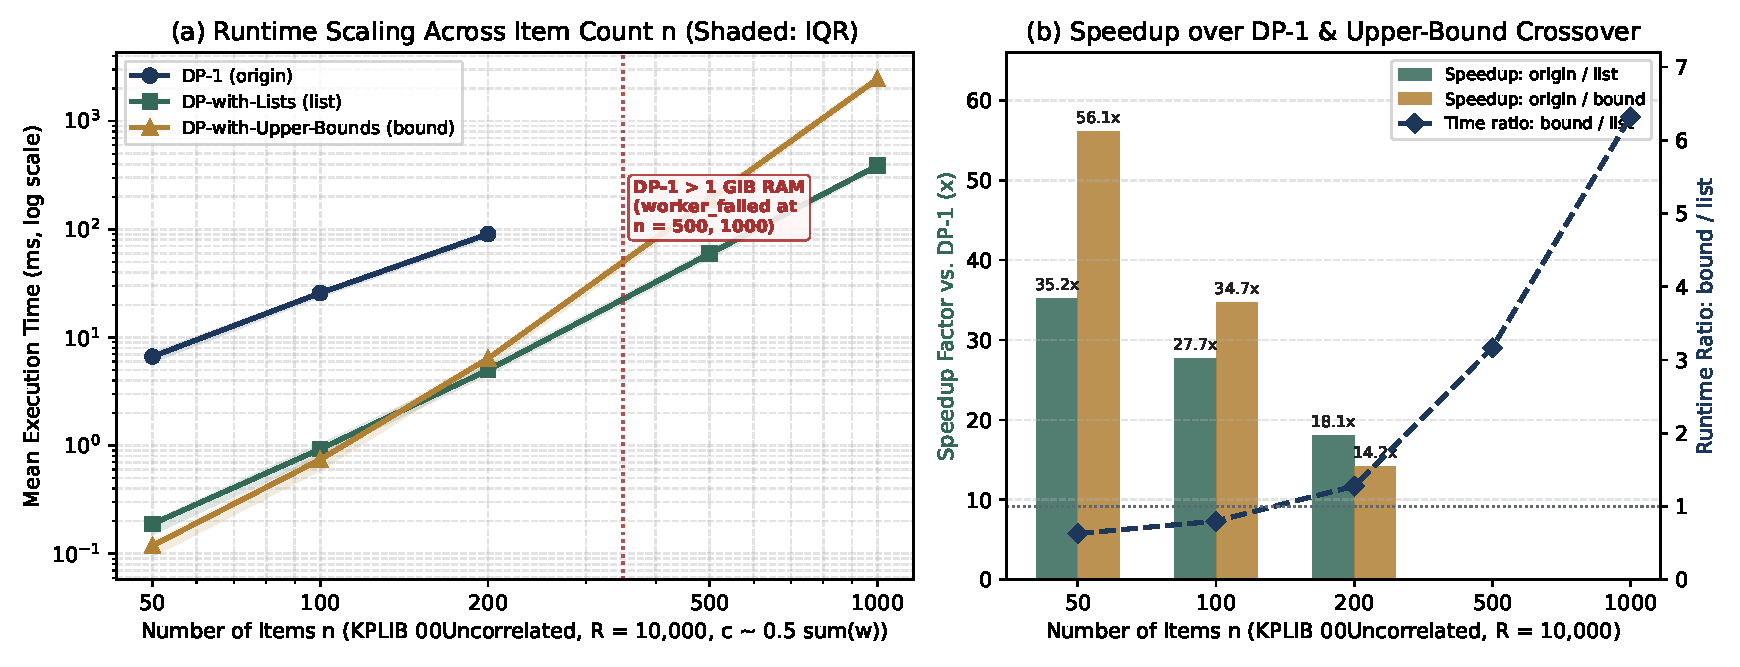
\includegraphics[width=0.98\textwidth]{scaling_r10000_overview.pdf}
\caption{\footnotesize Runtime scaling and speedup ratios on KPLIB \code{00Uncorrelated} at $R = 10{,}000$.}
\label{fig:r10k_overview}
\end{figure}

\vspace{-0.2em}
\begin{figure}[H]
\centering
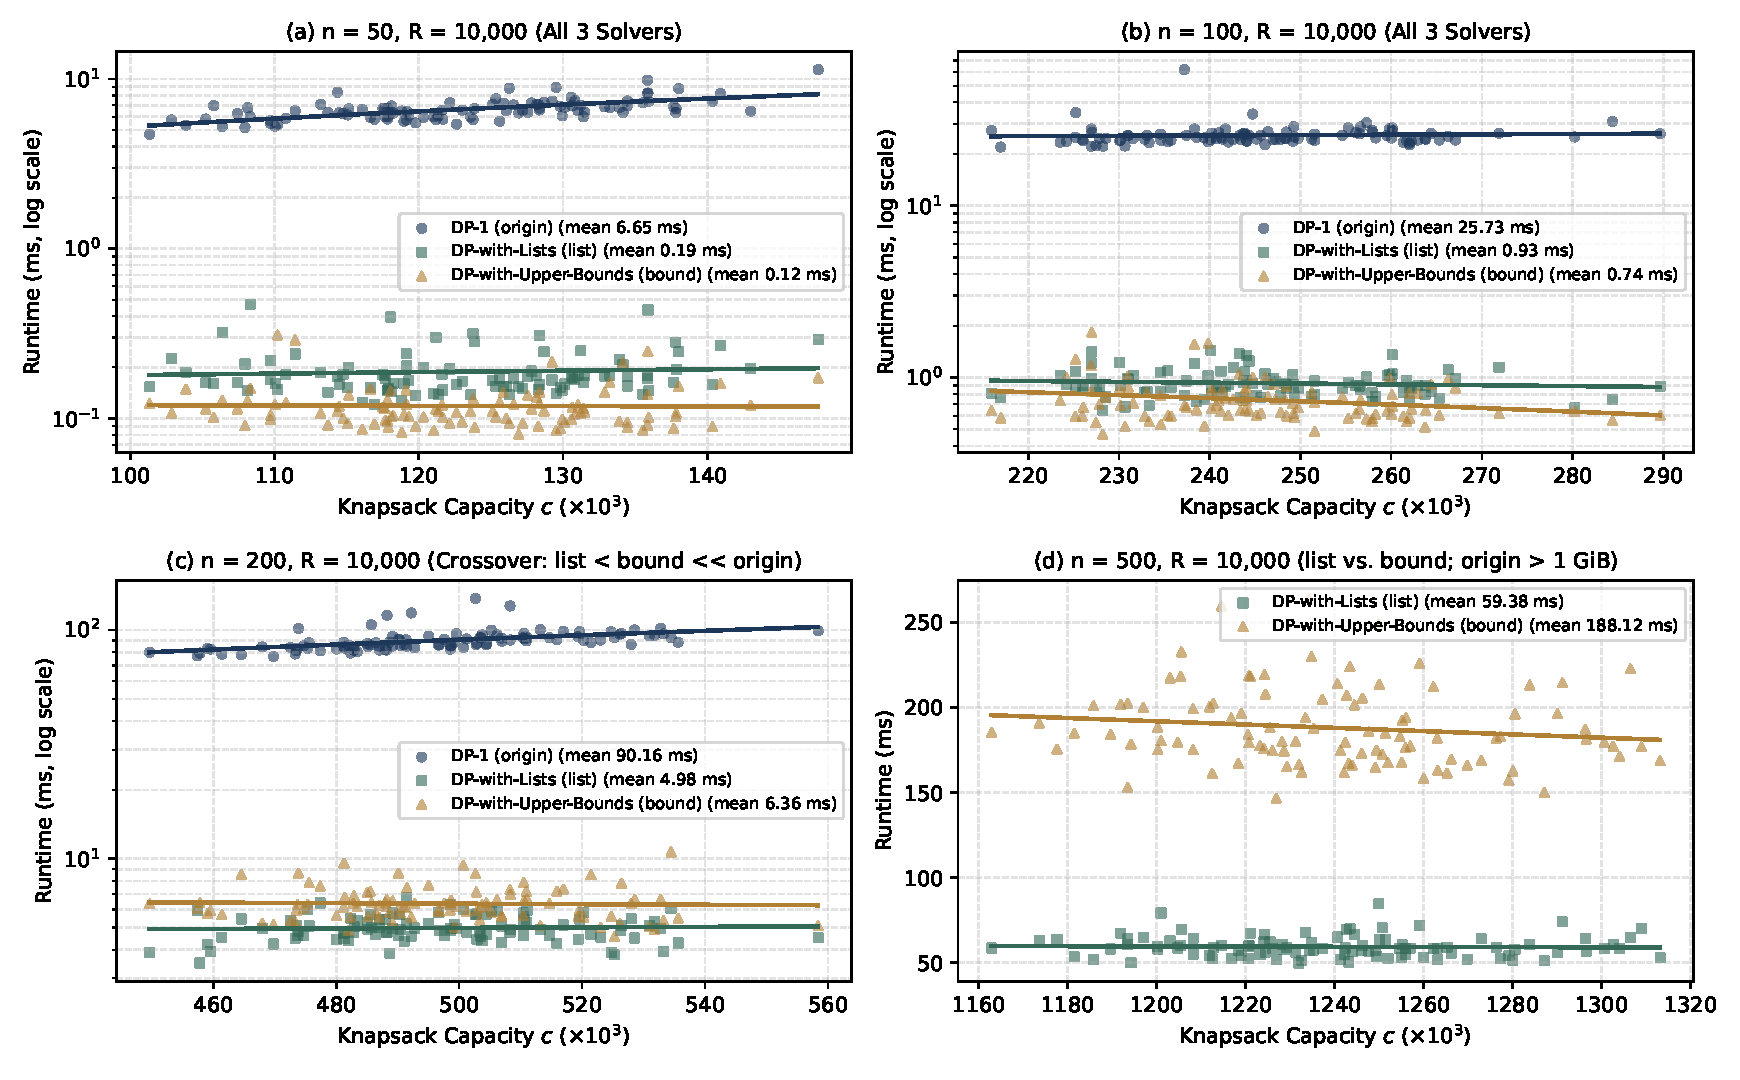
\includegraphics[width=0.98\textwidth]{runtime_vs_capacity_r10000.pdf}
\caption{\footnotesize Per-instance runtime versus capacity $c$ across four KPLIB scales at $R = 10{,}000$.}
\label{fig:r10k_cap}
\end{figure}

\vspace{-0.2em}
\begin{figure}[H]
\centering
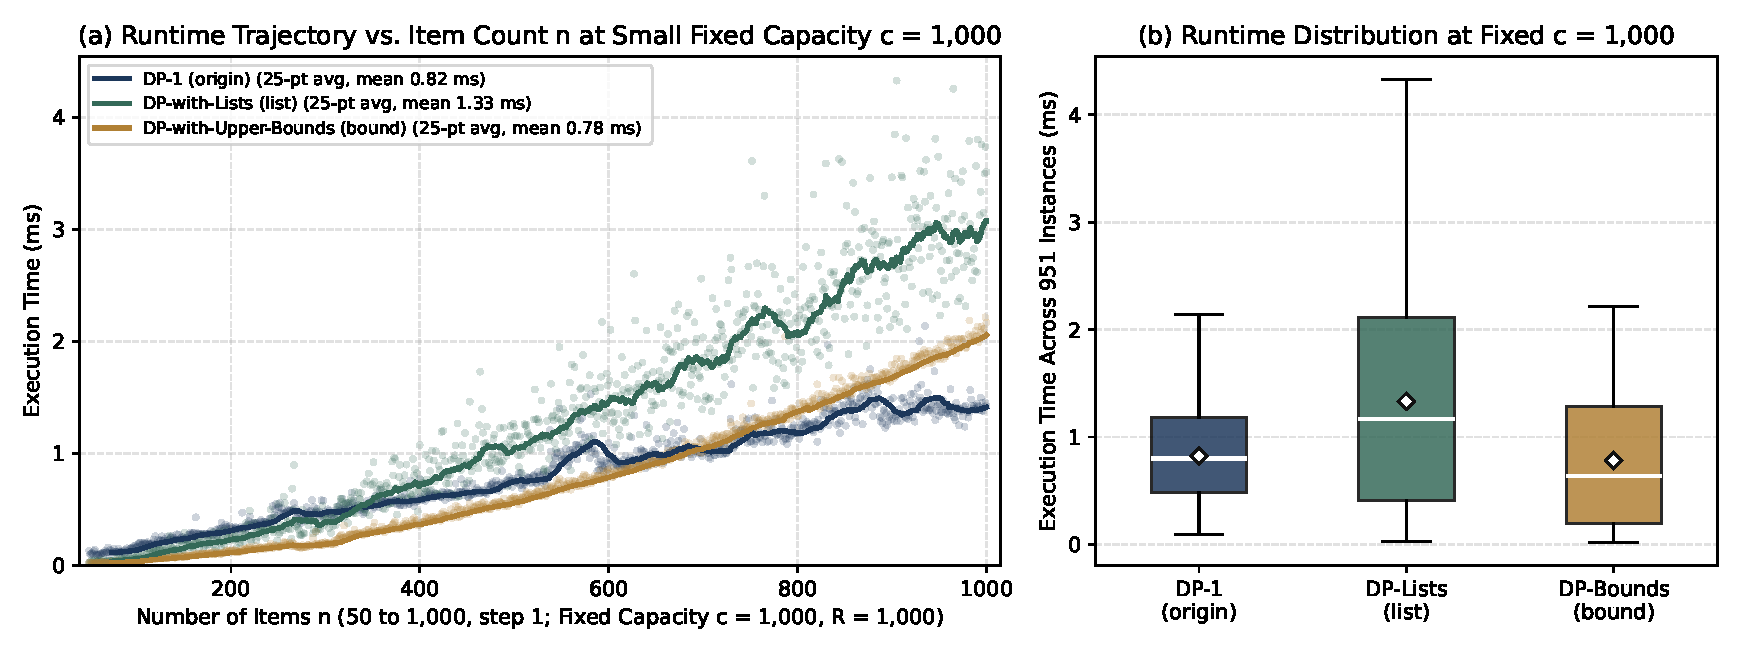
\includegraphics[width=0.98\textwidth]{runtime_vs_n_fixed_c1000.pdf}
\caption{\footnotesize Runtime trajectory and distribution across $n \in [50, 1000]$ at fixed $c = 1{,}000$.}
\label{fig:c1000_n}
\end{figure}

\vspace{-0.2em}
\begin{figure}[H]
\centering
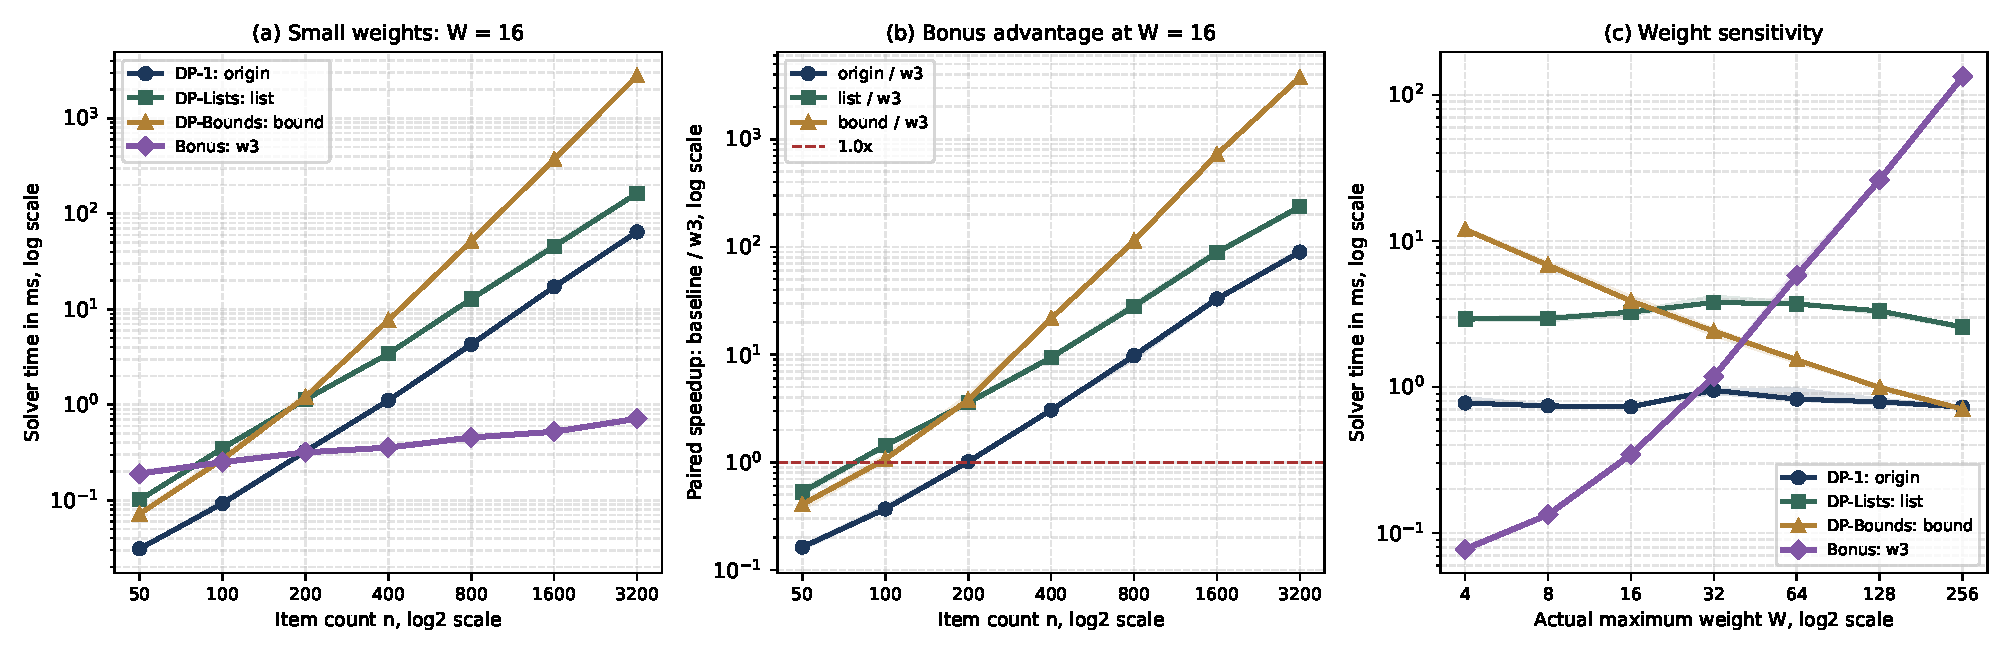
\includegraphics[width=0.99\textwidth]{bonus_regimes_overview.pdf}
\caption{\footnotesize Small-weight scaling at $W = 16$, paired speedups over \code{w3}, and weight sensitivity up to $W = 256$.}
\label{fig:bonus_regimes}
\end{figure}

\clearpage

% ============================================================
%  CHAPTER 4: ANALYSIS AND COMMENTS
% ============================================================
\section{Analysis and Comments}

\subsection{Time and Space Complexity Analysis}
Let $B = \max_{0 \le j \le n} |L_j| \le c + 1$ denote the maximum number of undominated states in any stage of \code{list}, $B_{\text{ub}} = \max_{0 \le j \le n} |L_j^{\text{ub}}| \le B$ denote the peak list length retained after upper-bound pruning in \code{bound}, and $W = \max_{1 \le j \le n} w_j$ denote the maximum usable item weight in \code{w3}. \Cref{tab:complexities} summarizes both the asymptotic bounds of our C11 implementations and the space-optimized rolling-buffer bounds.

\begin{table}[H]
\centering
\caption{Time and space complexities of the four exact 0/1 knapsack solvers.}
\label{tab:complexities}
\setlength{\tabcolsep}{3.1pt}
\footnotesize
\begin{tabular}{@{}lccccc@{}}
\toprule
\textbf{\color{primary}Algorithm} & \textbf{\color{primary}Best Time} & \textbf{\color{primary}Param.\ Time} & \textbf{\color{primary}Worst Time} & \textbf{\color{primary}C Impl.\ Space} & \textbf{\color{primary}Rolling Space} \\
\midrule
\textbf{DP-1}, \code{origin} & $\Theta(nc)$ & $\Theta(nc)$ & $\Theta(nc)$ & $\Theta(nc)$ & $\Theta(c)$ \\
\textbf{DP-Lists}, \code{list} & $\Theta(n)$ & $O(nB)$ & $O(nc)$ & $O(nB + c)$ & $O(B)$ \\
\textbf{DP-Bounds}, \code{bound} & $\Theta(n^2)$ & $O(n^2 + n^2 B_{\text{ub}})$ & $O(n^2 c)$ & $O(n B_{\text{ub}} + c + n)$ & $O(B_{\text{ub}} + n)$ \\
\textbf{Bonus SMAWK}, \code{w3} & $\Theta(n)$ & $O(n + W^3)$ & $O(n + W^3)$ & $O(n + W^2)$ & $O(n + W^2)$ \\
\bottomrule
\end{tabular}
\end{table}

\begin{lemmabx}{Lemma 1: Total Ordering and $O(nB)$ Bound of \textsf{DP-with-Lists} \cite{kellerer2004knapsack}}
Every undominated state list $L_j$ produced by \id{Mergelist} satisfies $0 \le w_{1j} < \cdots < w_{m_j,j} \le c$ and $0 \le p_{1j} < \cdots < p_{m_j,j}$, with $m_j = |L_j| \le \min(2^j, c+1)$. If $m_j \le B$ for all $j$, \code{knapsack\_list} runs in $O(nB)$ time and achieves $\Theta(n)$ best-case time.
\end{lemmabx}

\begin{proof}
Suppose two retained states $(w_a, p_a)$ and $(w_b, p_b)$ appear in $L_j$ with $a < b$. Because \id{Mergelist} pops candidates in non-decreasing weight order and replaces the tail whenever an equal weight improves profit, $w_a < w_b$ holds strictly. Meanwhile, Step~4 admits $(w_b, p_b)$ only when $p_b > p_a$, proving strict monotonicity in both coordinates and bounding $m_j \le c + 1$ since distinct integers in $[0, c]$ number at most $c + 1$.

At stage $j$, forming $L'_j$ scans at most $m_{j-1}$ states in $O(B)$ time, and \id{Mergelist} advances either cursor $i_1$ or $i_2$ at every iteration in $O(1)$ time, taking $O(|L_{j-1}| + |L'_j|) = O(B)$ time. Summing over $j = 1, \ldots, n$ yields $O(nB) \subseteq O(nc)$ time. In the best case---for example when $w_j = c$ for every item---each shifted state $(c + w_j, p + p_j)$ exceeds $c$ except $(c, p_j)$, so $|L_j| \le 2$ for all $j$ and total runtime drops to $\Theta(n)$.
\end{proof}

\begin{theorembx}{Theorem 1: Exactness and Complexity of \textsf{DP-with-Upper-Bounds} \cite{kellerer2004knapsack}}
With items sorted so $p_1/w_1 \ge \cdots \ge p_n/w_n$, the floored fractional-knapsack bound $U_j(w, p)$ in (\ref{eq:ub}) satisfies $z^* \ge P^*$ and $U_j(w, p) \ge p + \max\{\sum_{\ell=j+1}^n p_\ell x_\ell \mid \sum_{\ell=j+1}^n w_\ell x_\ell \le c - w,\; x_\ell \in \{0,1\}\}$. Hence fathoming states with $U_j(w, p) \le P^*$ preserves exactness of $z^*$, and \code{knapsack\_list\_with\_bound} runs in $O(n^2 + n^2 B_{\text{ub}}) \subseteq O(n^2 c)$ worst-case time.
\end{theorembx}

\begin{proof}
Because items are sorted in non-increasing order of $p_\ell / w_\ell$, greedy fractional packing solves the continuous relaxation $x_\ell \in [0,1]$ over residual capacity $c - w$ optimally. Relaxing $x_\ell \in \{0,1\}$ to $[0,1]$ cannot decrease the objective, and since all $p_\ell \in \mathbb{Z}_{\ge 0}$, any feasible integer completion has an integer profit at most $\lfloor U_j^{\text{LP}}(w, p) \rfloor = U_j(w, p)$. Whenever $U_j(w, p) \le P^*$, no binary extension of $(w, p)$ can strictly beat the already realized integer profit $P^*$, so discarding $(w, p)$ never eliminates all optimal solutions; if the optimal solution itself was already recorded in $P^*$, returning $P^*$ at termination remains exact.

For time complexity, \code{selection\_sort} takes $\Theta(n^2)$ preprocessing time. At stage $j$, the bounded merge step pops at most $2|L_{j-1}^{\text{ub}}| \le 2B_{\text{ub}}$ states, invoking \code{fraction\_knapsack} in $O(n - j)$ time per popped state. Summing over $j = 1, \ldots, n$ gives
\[
  T_{\text{bound}}(n, c) \;=\; \Theta(n^2) + \sum_{j=1}^{n} O\bigl((n - j + 1)\,|L_{j-1}^{\text{ub}}|\bigr) \;=\; O(n^2 + n^2 B_{\text{ub}}) \;\subseteq\; O(n^2 c).
\]
In the best case where the greedy prefix immediately fills capacity $c$ and prunes all suboptimal branches so $B_{\text{ub}} = O(1)$, total time drops to $\Theta(n^2)$ due to selection sort.
\end{proof}

\paragraph{Complexity of Bonus Solver \code{w3}.}
Given the $2W$ proximity bound from~\cite{polak2021knapsack}, filtering, geometric BFPRT prefix construction, and bucketing by weight each run in $O(n)$ time. Across weights $h \in \{1, \ldots, W\}$, keeping at most $2W$ items per group retains $O(W^2)$ items in total, so sorting them takes $O(W^2 \log W)$ time. For each weight $h$, residue class $r \in \{0, \ldots, h - 1\}$ has $O(W^2 / h)$ indices in $[0, L + \Delta]$, so \code{kw3\_smawk} takes $\sum_{r=0}^{h-1} O(W^2 / h) = O(W^2)$ time per weight and $O(W^3)$ time across at most $W$ weights, while recombining $D$ and $A_{\le}$ takes $O(W^2)$. Thus \code{knapsack\_w3} runs in $O(n + W^3)$ time and uses $O(n + W^2)$ auxiliary space without allocating capacity-$c$ tables.

\paragraph{Byte-Level Space Accounting and Memory Regimes.}
In \code{Knapsack\_origin.h}, \code{best\_solution} allocates $(n+1)(c+1)$ 4-byte integers plus row pointers:
\begin{itemize}
  \item \textbf{Dense Table \code{origin}:} Uses $380.8\,\text{MiB}$ at $n = 200, c = 496{,}705$, but demands $\mathbf{2.31\,\text{GiB}}$ at $n = 500$ and $\mathbf{9.22\,\text{GiB}}$ at $n = 1{,}000$, exceeding the $1\,\text{GiB}$ Job cap across all $200$ instances in TC-4 and TC-5.
  \item \textbf{State Lists \code{list} and \code{bound}:} Each \code{State} takes $8$ bytes; $|L_j| \ll c$ lets $99/100$ \code{list} runs and $100/100$ \code{bound} runs finish within $1\,\text{GiB}$ at $n = 1{,}000$, with one OOM on \code{s061.kp} from retaining $L_{0..n}$.
  \item \textbf{Bonus \code{w3}:} Allocates $O(n + W^2)$ arrays of length $\le 2W^2 + W + 1$, using under $0.15\,\text{MiB}$ at $W = 16, n = 3{,}200$, versus $\approx 112\,\text{MiB}$ when $W \approx 1{,}000$ makes $L \approx 2\times 10^6$.
\end{itemize}

\subsection{Empirical Performance Insights Across Regimes}
Four key findings explain the empirical speedups and regime crossovers observed across all benchmarks in Chapter~3.

\vspace{-0.3em}
\begin{insightbox}{Key Finding 1: Undominated State Pruning Yields $14\times\text{--}56\times$ Speedups on Large Capacities}
When item weights are drawn uniformly from $[1, 10{,}000]$ at $n \in \{50, 100, 200\}$, capacity $c \approx 2{,}500n$ reaches $1.2 \times 10^5$ to $5.0 \times 10^5$, forcing \textbf{DP-1} to fill $6.2 \times 10^6$ to $1.0 \times 10^8$ table cells. In early and middle stages, reachable weight sums remain sparse and high-density items dominate nearby weight combinations. Because $B \ll c$, \code{list} cuts mean runtime from $90.16\,\text{ms}$ to $4.98\,\text{ms}$ by $\mathbf{18.10\times}$ at $n=200$, and \code{bound} cuts mean runtime from $6.65\,\text{ms}$ to $0.12\,\text{ms}$ by $\mathbf{56.08\times}$ at $n=50$. At $n=1{,}000$, \code{list} and \code{bound} average $0.39\,\text{s}$ and $2.45\,\text{s}$, whereas dense-table DP exceeds $1\,\text{GiB}$ of RAM.
\end{insightbox}
\vspace{-0.35em}

\begin{insightbox}{Key Finding 2: Per-State $O(n)$ Bounding Causes the $n \approx 150$ Crossover on Large $R$}
Comparing \code{list} and \code{bound} on KPLIB in \Cref{tab:r10000,fig:r10k_overview} shows a clear trade-off between state reduction and per-state bounding cost:
\begin{itemize}
  \item \textbf{Small $n \le 100$:} Each \code{fraction\_knapsack} call scans fewer than $100$ contiguous integers in L1 cache while pruning over half of the candidate states, raising the speedup over \textbf{DP-1} from $35.25\times$ to $56.08\times$ at $n=50$.
  \item \textbf{Large $n \in \{500, 1000\}$:} Once high-ratio items are packed, thousands of states still satisfy $U_j(w,p) > P^*$. Running an $O(n - j)$ scan on every merged state pushes \code{bound} toward its $O(n^2 B_{\text{ub}})$ bound, raising median runtime at $n=1{,}000$ from $382.89\,\text{ms}$ for \code{list} to $2{,}416.38\,\text{ms}$ for \code{bound}, while \code{bound}'s smaller lists avoid the single OOM on \code{s061.kp}.
\end{itemize}
\end{insightbox}
\vspace{-0.35em}

\begin{insightbox}{Key Finding 3: Cache-Friendly Dense Arrays Beat Unbounded Lists When Capacity $c$ Is Small}
At fixed $c = 1{,}000$ and $n \in [50, 1000]$ in \Cref{tab:c1000,fig:c1000_n}, $B$ quickly approaches $c = 1{,}000$. Without upper-bound pruning, \code{list} loses its sparsity advantage: per-stage \code{malloc}/\code{free} calls, merge branches in \code{Mergelist}, and 8-byte struct copies make \code{list} nearly $2\times$ slower than \code{origin}'s sequential \code{int} loop for $n \in [800, 1000]$, averaging $2.76\,\text{ms}$ versus $1.40\,\text{ms}$. Upper-bound pruning in \code{bound} keeps lists short for $n < 600$ and wins $640/951$ instances overall, whereas \code{selection\_sort} and $O(n-j)$ bounding let \code{origin} take the lead for $n \ge 650$.
\end{insightbox}
\vspace{-0.35em}

\begin{insightbox}{Key Finding 4: Bonus \code{w3} Excels at Small $W$ and Large $n$ but Degrades Rapidly at Large $W$}
At fixed $W = 16$ in \Cref{tab:bonus,fig:bonus_regimes}, each correction array has fixed length $\approx 2W^2 = 512$ independent of $n$ and $c$, while preprocessing stays linear in $n$; thus \code{w3} takes only $\mathbf{0.716\,\text{ms}}$ at $n = 3{,}200$ while \code{origin} grows with $nc$, \code{list} grows with reachable states, and \code{bound} pays selection-sort and per-state scan overhead. Conversely, when $W$ is large at small or moderate $n$, scanning a $2W^2$ window per distinct weight with BFPRT and SMAWK overhead dominates: \code{w3} rises to $133.39\,\text{ms}$ at $W = 256$ and $390.14\,\text{ms}$ on KPLIB $n = 50, W \approx 989$, where $2W^2 \approx 2\times 10^6$ far exceeds median capacity $c = 12{,}340$.
\end{insightbox}
\vspace{-0.35em}

\subsection{Further Possible Improvements}
\vspace{-0.15em}
Based on our analysis and profiling, two improvements are planned for future work:
\begin{enumerate}[label=\textbf{\color{primary}\arabic*.}]
  \item \textbf{Rolling Array / Two-List Allocation:} Stage $j$ depends only on stage $j - 1$. Freeing $L_{j-1}$ right after building $L_j$, and replacing \code{best\_solution[n+1][c+1]} in \textbf{DP-1} with a single 1D array \code{dp[0..c]}, reduces space from $\Theta(nc)$ and $O(nB)$ to $\Theta(c)$ and $O(B)$, removing all $1\,\text{GiB}$ OOM failures at $n = 500$ and $1{,}000$.
  \item \textbf{Replacing Selection Sort with \code{qsort} and Pre-Sizing $L_0$:} Replacing $\Theta(n^2)$ \code{selection\_sort} with $\Theta(n \log n)$ \code{qsort} and starting $L_0$ with a small initial capacity instead of $c + 1$ avoids unnecessary upfront overhead at large $n$ and $c$.
\end{enumerate}

\clearpage

% ============================================================
%  AUTHOR LIST, DECLARATION, AND REFERENCES
% ============================================================
\section*{Author List and Declaration}
\addcontentsline{toc}{section}{Author List and Declaration}

\subsection*{Author List}
{\sloppy
\ifpeerreview
\begin{itemize}
  \item \textbf{\color{primary}Student A:} Implemented the four exact knapsack solvers \code{Knapsack\_origin.h}, \code{Knapsack\_List.h}, \code{Fraction\_Knapsack.h}, \code{Knapsack\_List\_with\_bound.h}, and \code{Knapsack\_w3.h}, regression driver \code{test\_w3.c}, benchmark harness \code{testbench.c}, and generator \code{knapsack\_generator.py}.
  \item \textbf{\color{primary}Student B:} Executed and verified the KPLIB, fixed-capacity, and bonus regime suites via \code{experiment\_bonus.py}, wrote the plotting scripts \code{plot\_benchmark.py} and \code{visualization.py}, conducted the complexity and crossover analysis, and authored this report.
\end{itemize}
\else
\begin{itemize}
  \item \textbf{\color{primary}Yixiang Chen:} Implemented the four exact knapsack solvers \code{Knapsack\_origin.h}, \code{Knapsack\_List.h}, \code{Fraction\_Knapsack.h}, \code{Knapsack\_List\_with\_bound.h}, and \code{Knapsack\_w3.h}, regression driver \code{test\_w3.c}, benchmark harness \code{testbench.c}, and generator \code{knapsack\_generator.py}.
  \item \textbf{\color{primary}Runhui Lin:} Executed and verified the KPLIB, fixed-capacity, and bonus regime suites via \code{experiment\_bonus.py}, wrote the plotting scripts \code{plot\_benchmark.py} and \code{visualization.py}, conducted the complexity and crossover analysis, and authored this report.
\end{itemize}
\fi
}

\subsection*{Declaration}
We hereby declare that all the work done in this project titled ``Improving Dynamic Programming for the 0/1 Knapsack Problem'' is of our independent effort as a group.

\subsection*{Signatures}
\vspace{0.35cm}
\noindent
\ifpeerreview
\begin{minipage}[t]{0.48\linewidth}
\centering
\vspace{1.15cm}
\rule{0.92\linewidth}{0.4pt}\\[0.15cm]
Student A
\end{minipage}\hfill
\begin{minipage}[t]{0.48\linewidth}
\centering
\vspace{1.15cm}
\rule{0.92\linewidth}{0.4pt}\\[0.15cm]
Student B
\end{minipage}
\else
\begin{minipage}[t]{0.48\linewidth}
\centering

\includegraphics[height=1.35cm,keepaspectratio]{signature_chen.png}\\[-0.1cm]
\rule{0.92\linewidth}{0.4pt}\\[0.15cm]
Yixiang Chen
\end{minipage}\hfill
\begin{minipage}[t]{0.48\linewidth}
\centering

\includegraphics[height=1.55cm,keepaspectratio]{signature_lin.png}\\[-0.1cm]
\rule{0.92\linewidth}{0.4pt}\\[0.15cm]
Runhui Lin
\end{minipage}
\fi

\vspace{0.6cm}
\printbibliography[heading=bibintoc]

\clearpage

% ============================================================
%  APPENDIX
% ============================================================
\appendix
\titleformat{\section}
  {\color{primary}\centering\Large\bfseries}
  {\color{accent}Appendix~\thesection.}{0.6em}{}
  [\vspace{0.3em}{\color{accent!70}\titlerule[1.5pt]}]

\section{Source Code}

All source files reside in \code{project4/src/} with over $30\%$ commented lines in every C11 source and header file. Below we list the four solver headers, the fractional-knapsack helper, the demo and regression drivers, the Job-Object benchmark harness, and the Python generation, bonus experiment, and visualization scripts.

\subsection{Baseline Dense-Table DP: \texttt{Knapsack\_origin.h}}
\lstinputlisting[language=C]{../src/Knapsack_origin.h}

\subsection{DP-with-Lists and Dominance Pruning: \texttt{Knapsack\_List.h}}
\lstinputlisting[language=C]{../src/Knapsack_List.h}

\subsection{Fractional Knapsack Upper-Bound Helper: \texttt{Fraction\_Knapsack.h}}
\lstinputlisting[language=C]{../src/Fraction_Knapsack.h}

\subsection{DP-with-Upper-Bounds: \texttt{Knapsack\_List\_with\_bound.h}}
\lstinputlisting[language=C]{../src/Knapsack_List_with_bound.h}

\subsection{Bonus \texorpdfstring{$O(n + W^3)$}{O(n + W3)} Proximity + SMAWK Solver: \texttt{Knapsack\_w3.h}}
\lstinputlisting[language=C]{../src/Knapsack_w3.h}

\subsection{Sanity-Check Demo Driver: \texttt{testbench\_demo.c}}
\lstinputlisting[language=C]{../src/testbench_demo.c}

\subsection{Deterministic Bonus Regression Suite: \texttt{test\_w3.c}}
\lstinputlisting[language=C]{../src/test_w3.c}

\subsection{Job-Object Batch Benchmark Harness: \texttt{testbench.c}}
\lstinputlisting[language=C]{../src/testbench.c}

\subsection{Reproducible Knapsack Instance Generator: \texttt{knapsack\_generator.py}}
\lstinputlisting[language=Python]{../src/knapsack_generator.py}

\subsection{Controlled Bonus Regime Runner: \texttt{experiment\_bonus.py}}
\lstinputlisting[language=Python]{../src/experiment_bonus.py}

\subsection{Benchmark Visualization Script: \texttt{visualization.py}}
\lstinputlisting[language=Python]{../src/visualization.py}

\end{document}
